In many areas around the world, air pollution is the leading environmental health risk affecting both the human population and ecology.
The effects of air pollution range from chronic to less severe health impacts to the general population, air pollution has been labelled carcinogenic by the International Agency for Research on Cancer \citep{IARC:2013}, significant economic impacts due to reduced growth rates of vegetation run into billions of euros per year.
Due to these impacts, many governed areas introduced limit values for the most common and severe air pollutants \citep{AQEU:2015}.

Air pollutants can be emitted directly into the atmosphere (\emph{primary pollutants}) or formed from the chemical reactions of other pollutants (\emph{secondary pollutants}).
Over Europe, particulate matter (PM) and tropospheric ozone (\ce{O3}) are the most problematic with up to $93$ and $98$~\% of Europe's urban population exposed to concentrations above the WHO guidelines \citep{AQEU:2015}.

Tackling the high levels of tropospheric ozone is a complex problem as it is secondary pollutant formed from the reactions of emitted nitrogen oxides (\ce{NO_x}~$\equiv$~NO + \ce{NO2}) and volatile organic compounds (VOCs) in the presence of sunlight.
The photochemical nature of ozone production also lends itself to large impacts from meteorological variables such as temperature and wind speed \citep{Jacob:2009}.
Despite reductions to ozone precursors, the EU target value for human health (the EU does not currently have a  limit value for ozone) was exceeded in $65$~\% of the EU member states and Europe's target value for vegetation was exceeded in $27$~\% of the EU-28 agricultural areas \citep{AQEU:2013}.

Air quality (AQ) modelling is an important tool for predicting future air quality under different emission and meteorological scenarios.
Adequately representing the complexity of ozone production is an ongoing challenge for the modelling community.
Representing the numerous inputs in a correct way that is computationally efficient to reproduce observed trends in tropospheric ozone is a challenge for AQ models.

In this work, we shall determine the effects of different representations of specific model inputs on simulated ozone production.
The research questions addressed in this work, relate specifically to the representation of chemistry, inputs of VOC emissions and temperature on ozone production and are detailed further in Sect.~\ref{s:research_questions}.
After determining the effects on ozone production, Chap.~\ref{c:conclusions} frames these effects in the wider view of improving current state of the art AQ modelling of tropospheric ozone.

\section{Ozone} \label{s:ozone}
%atmospheric O3 with budget, lifetime, stratospheric & tropospheric ozone
Ozone is a constituent gas of the atmosphere found in the stratosphere and troposphere, however its atmospheric effects are very different in these distinct regions.
About 90~\% of the atmospheric ozone is present in the stratosphere with a peak mixing ratio of about $12$~ppm \citep{Seinfeld:2006}.
Stratospheric ozone absorbs the sun's ultraviolet radiation with wavelengths between $280$ and $315$~nm, this is extremely important as excess UV radiation may cause skin cancer, cataracts and a suppressed immune system in humans and can also damage land and aquatic ecosystems \citep{WMO:2010}. 

In contrast, tropospheric ozone, found close to the surface, is both a pollutant and a greenhouse gas. 
Increased levels of tropospheric ozone are harmful to humans, plants and other living systems, as high ozone exposure can lead to pulmonary problems in humans and can decrease both crop yields and forest growth \citep{WMO:2010}. 

Globally, tropospheric ozone is formed mainly via photochemical production from the reactions of emitted VOCs and \ce{NO_x}.
However, the Statospere-Troposphere Exchange (STE), which transports ozone from the stratosphere into the troposphere, may also play a role. 
The STE is driven by the Brewer-Dobson circulation \citep{Brewer:1949, Dobson:1956}, a relatively slow circulation (weeks to months) due to planetary wave disturbances in the troposphere \citep{Haynes:1991}.
The circulation causes air to move downward from the stratosphere into the troposphere at the mid and high latitudes and is balanced by upward exchange at the tropics. 
%The STE also has a seasonal variability where the maximum transport occurs during spring \citep{Appenzeller:1996}, due to the increase in altitude of the tropopause - the boundary level between the troposphere and the stratosphere - which moves stratospheric air into the troposphere. 

A spring-time peak in \ce{O3} concentrations is common in the mid-latitudes of the Northern Hemisphere and the STE was thought to be responsible. 
However, it is only very rarely that \ce{O3} originating via STE can influence tropospheric \ce{O3} levels \citep{Lelieveld:2000}. 
It was later realised that this spring maximum is due to the photochemical reactions occuring in the Northern Hemisphere spring after the buildup of reservoir species over winter \citep{Penkett:1986}.
These reservoir species are oxidised photochemically at a faster rate due to the increase in temperature, moisture and sunlight.

%metereology impacts 
Tropospheric \ce{O3} is not only impacted by emission levels, it is also affected by meteorological variables such as temperature, number of hours of sunshine and wind as these impact transport, dry and wet deposition rates and also chemical reaction rates \citep{Hess:2009}.
Meteorology influences both regional and global \ce{O3} \citep{Hess:2009}, climate patterns such as El Ni\~{n}o are also known to impact \ce{O3} levels in certain areas \citep{Sudo:2001}. 
The effects of meteorology on ozone production shall be presented in more detail in Sect.~\ref{s:meteo_ozone}.

In general, there has been great effort to reduce emissions of ozone precursors from anthropogenic sources.
For example, the emissions of non-methane VOCs (NMVOCs) over Europe have decreased by $20$~\% and emissions of \ce{NO_x} have decreased by almost $30$~\% from 2004 levels.
Despite these reductions in ozone precursors, up to $98$~\% of Europe's urban population are exposed to levels of ozone exceeding the WHO guidelines \citep{AQEU:2015}.

Modelling of \ce{O3} production has played a part in understanding the complexity of atmospheric chemistry, such as the non-linear relationship of \ce{O3} production on the concentrations of VOCs and \ce{NO_x}.
The results of these modelling experiments can be used to produce more effective strategies for reducing ozone levels.
The need for more effective air quality standards in turn also drives the model development and deeper understanding of the atmospheric processes controlling ozone production.
In this work, we shall address the representation of three important parts of an AQ model (chemistry, NMVOC emissions and meteorology) and their impacts on simulated ozone production.

\section{Ozone Production Chemistry} \label{s:ozone_chemistry}
%O3 chemical sources & sinks, linking VOCs.
Ozone is chemically produced and destroyed through the null photochemical cycle involving nitrogen dioxide (\ce{NO2}) and nitrogen oxide (NO) in Reactions~\eqref{r:NO2_hv}, \eqref{r:O_O2} and \eqref{r:NO_O3}.
This null cycle produces net ozone with the presence of VOCs of both biogenic and anthropogenic origin in the atmosphere. 
Secondary degradation products of the emitted VOCs, in the presence of \ce{NO_x}, react with NO to produce \ce{NO2}.
In the presence of sunlight, the newly-formed \ce{NO2} photolyses via \eqref{r:NO2_hv} producing ozone through \eqref{r:O_O2}.
\begin{rxnarray}
    \ce{NO2 + h\nu} & \rightarrow \ce{NO + O(^3P)} \label{r:NO2_hv} \\
    \ce{O(^3P) + O2} & \xrightarrow[]{\text{\tiny{M}}} \ce{O3} \label{r:O_O2} \\
    \ce{NO + O3} & \rightarrow \ce{NO2 + O2} \label{r:NO_O3}
\end{rxnarray}

%atmospheric chemistry of NMVOCs 
Many thousands of VOCs are emitted into the atmosphere from anthropogenic and biogenic sources, discussed further in Sect.~\ref{s:precursor_emissions}. 
Despite the vast array of VOCs, there are many common features between the degradation pathways.
Figure~\ref{f:VOC_reaction} represents a general and simplified reaction scheme for VOCs in the troposphere. 
\begin{figure}[t]
    \begin{center}
        \caption[Schematic of general secondary degradation of VOCs]{Schematic diagram outlining general pathways of the secondary degradation of an emitted VOC.}
        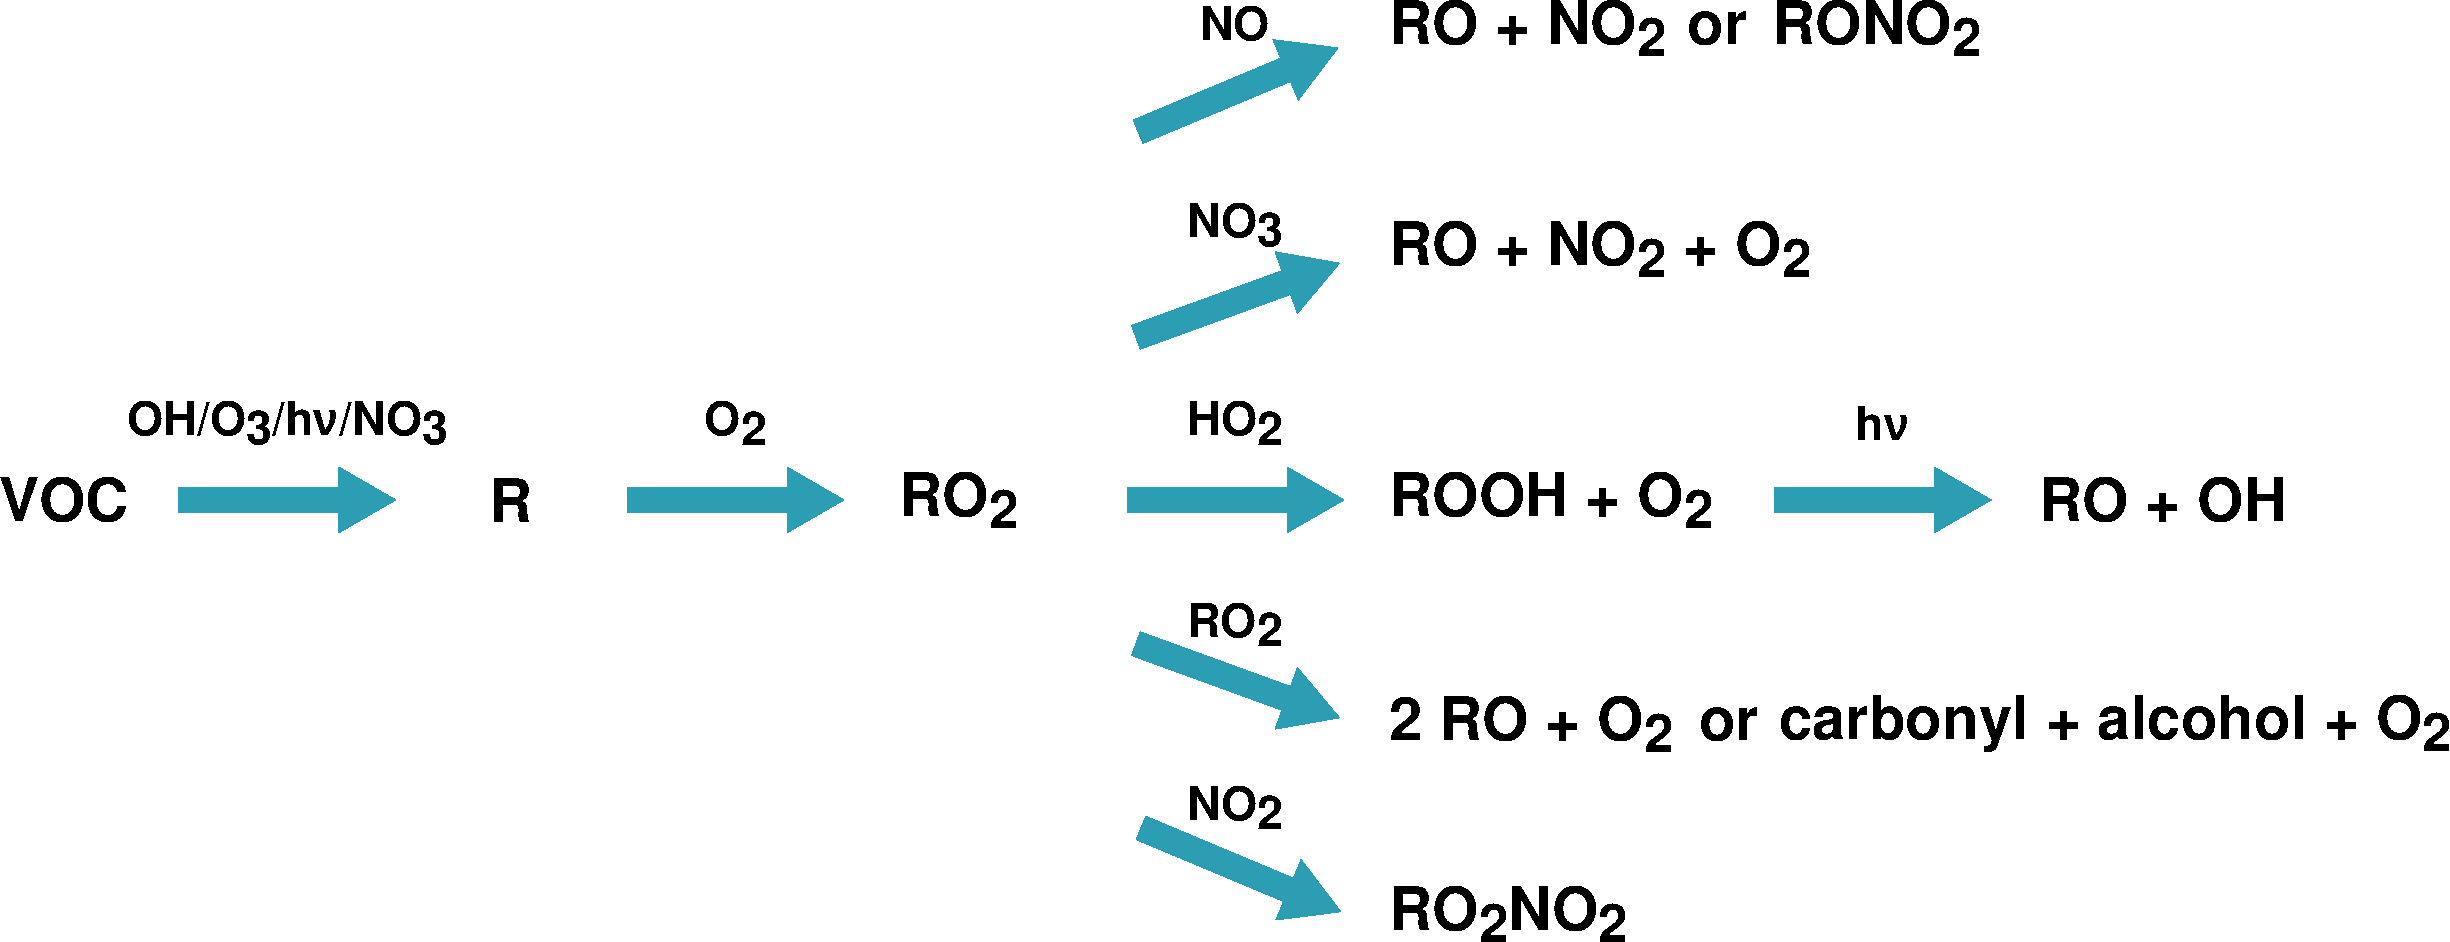
\includegraphics[width = \textwidth]{VOC_degradation}
        \label{f:VOC_reaction}
    \end{center}
\end{figure}

The primary oxidation of a VOC is typically through reaction with the hydroxyl (OH) radical.
Ozone also plays an important role in the production of OH radicals.
The photolysis of ozone \eqref{r:O3_hv} at wavelengths less than $335$~nm produces excited oxygen atoms (\ce{O^1D}) which when reacting with water vapour produce OH \eqref{r:O1D_H2O}.
\begin{rxnarray}
    \ce{O3 + h\nu} & \rightarrow \ce{O2 + O^1D} \label{r:O3_hv} \\
    \ce{O^1D + H2O} & \rightarrow \ce{2 OH} \label{r:O1D_H2O}
\end{rxnarray}

The reaction of a VOC with OH forms an alkyl or substituted alkyl radical (R) which in the presence of \ce{O2} produces alkyl peroxy radicals (\ce{RO2}).
Unsaturated VOCs, such as alkenes, may also react with ozone while photolysis is a primary degradation pathways for carbonyl species.
During the night-time, reaction with the \ce{NO3} radical is of importance.
These initial reaction pathways all lead to the formation of \ce{RO2} radicals.
\begin{rxnarray}
    \ce{VOC + OH / NO3 / O3 / h\nu} & \rightarrow \ce{R} \label{r:VOC_init} \\
    \ce{R + O2} & \rightarrow \ce{RO2} \label{r:R_O2}
\end{rxnarray} 

\ce{RO2} radicals can subsequently react with NO, \ce{NO2}, hydroperoxy (\ce{HO2}) radicals, \ce{NO3} radicals - mainly during night-time - and with other alkyl peroxy radicals \citep{Atkinson:2000}. 
The competition between these reactions, especially those pathways involving \ce{NO_x} (\eqref{r:RO2_NOa}, \eqref{r:RO2_NOa} and \eqref{r:RO2_NO2}), determines the amount of net production or loss of ozone. 
\begin{rxnarray}
    \ce{RO2 + NO} & \xrightarrow[]{\text{M}} \ce{RONO2} \label{r:RO2_NOa} \\
    \ce{RO2 + NO} & \rightarrow \ce{RO + NO2} \label{r:RO2_NOb} \\
    \ce{RO2 + NO2} & \xrightleftharpoons[]{\text{M}} \ce{RO2NO2} \label{r:RO2_NO2} \\
    \ce{RO2 + HO2} & \rightarrow \ce{ROOH + O2} \label{r:RO2_HO2} \\
    \ce{RO2 + NO3} & \rightarrow \ce{RO + NO2 + O2} \label{r:RO2_NO3} \\
    \ce{RO2 + RO2} & \rightarrow \ce{2RO + O2} \label{r:RO2_RO2a} \\
    \ce{RO2 + RO2} & \rightarrow \ce{RCH(OH)R + RC(O)R + O2} \label{r:RO2_RO2b}
\end{rxnarray}
All reactions pathways of \ce{RO2} that produce \ce{NO2} can result in \ce{O3} formation due to \eqref{r:NO2_hv} and \eqref{r:O_O2}. 
Reaction with the \ce{HO2} radical forms a hydroperoxide (ROOH) which then photolyses producing an alkoxy (RO) radical and recycling an OH radical.
The carbonyl and alcohol products resulting from reaction with other \ce{RO2} radicals will follow a similar sequence of reactions and hence can also produce further \ce{O3}. 
Thus the secondary degradation products of a VOC may also lead to further production of ozone.

Reaction of \ce{RO2} with \ce{NO2} leads to the formation of peroxynitrates (\ce{RO2NO2}) which are a temporary reservoir for \ce{RO2} and \ce{NO_x}.
When temperatures are low, the thermal decomposition of \ce{RO2NO2} to recycle \ce{RO2} and \ce{NO_x} happens at a slower rate than at higher temperatures.
Hence, at lower temperatures these \ce{RO2NO2} may build up and be transported away from their region of formation and re-release \ce{RO2} and \ce{NO2} downwind fuelling ozone production away from large sources of \ce{NO_x}.
This is one example of the dependence of ozone production on meteorogological variables, a broader overview is given in Sect.~\ref{s:meteo_ozone}.

The secondary degradation of the RO radical formed from many of the \ce{RO2} reactions proceeds through either decomposition, isomerisation or reaction with \ce{O2}. 
The products that result from the reaction pathways depend on the parent VOC and this also determines the number of NO-to-\ce{NO2} conversions, eventually leading to \ce{O3} formation.

The final degradation products of VOCs are carbon dioxide (\ce{CO2}) and water vapour. 
The path that each VOC takes to reach its final products is dependent on the type of VOC, the radical concentration, the \ce{NO_x} concentration and other factors such as time of day and year. 
The detailed atmospheric chemistry of most VOCs is well-understood however for more complex VOCs the complete set of reaction pathways of all the secondary degradation products there are a great number of uncertainties. 
These uncertainties may be related to kinetic data, photolysis rates, reaction branching ratios and in most cases the reaction products.
Any uncertainties in reaction pathways and products of VOCs also leads to uncertainties in estimating the amount of ozone produced during the degradation of a particular VOC \citep{Atkinson:2000}.

\subsection[VOC and NOx Chemistry]{VOC and \ce{NO_x} Chemistry} \label{ss:VOC&NOx}
\begin{figure}
	\begin{center}
        \caption[Ozone mixing ratios as a function of \ce{NO_x} and VOC]{Ozone isopleth plots for various initial mixing ratios of \ce{NO_x} and a VOCs. taken from \citet{Jenkin:2000}.}
        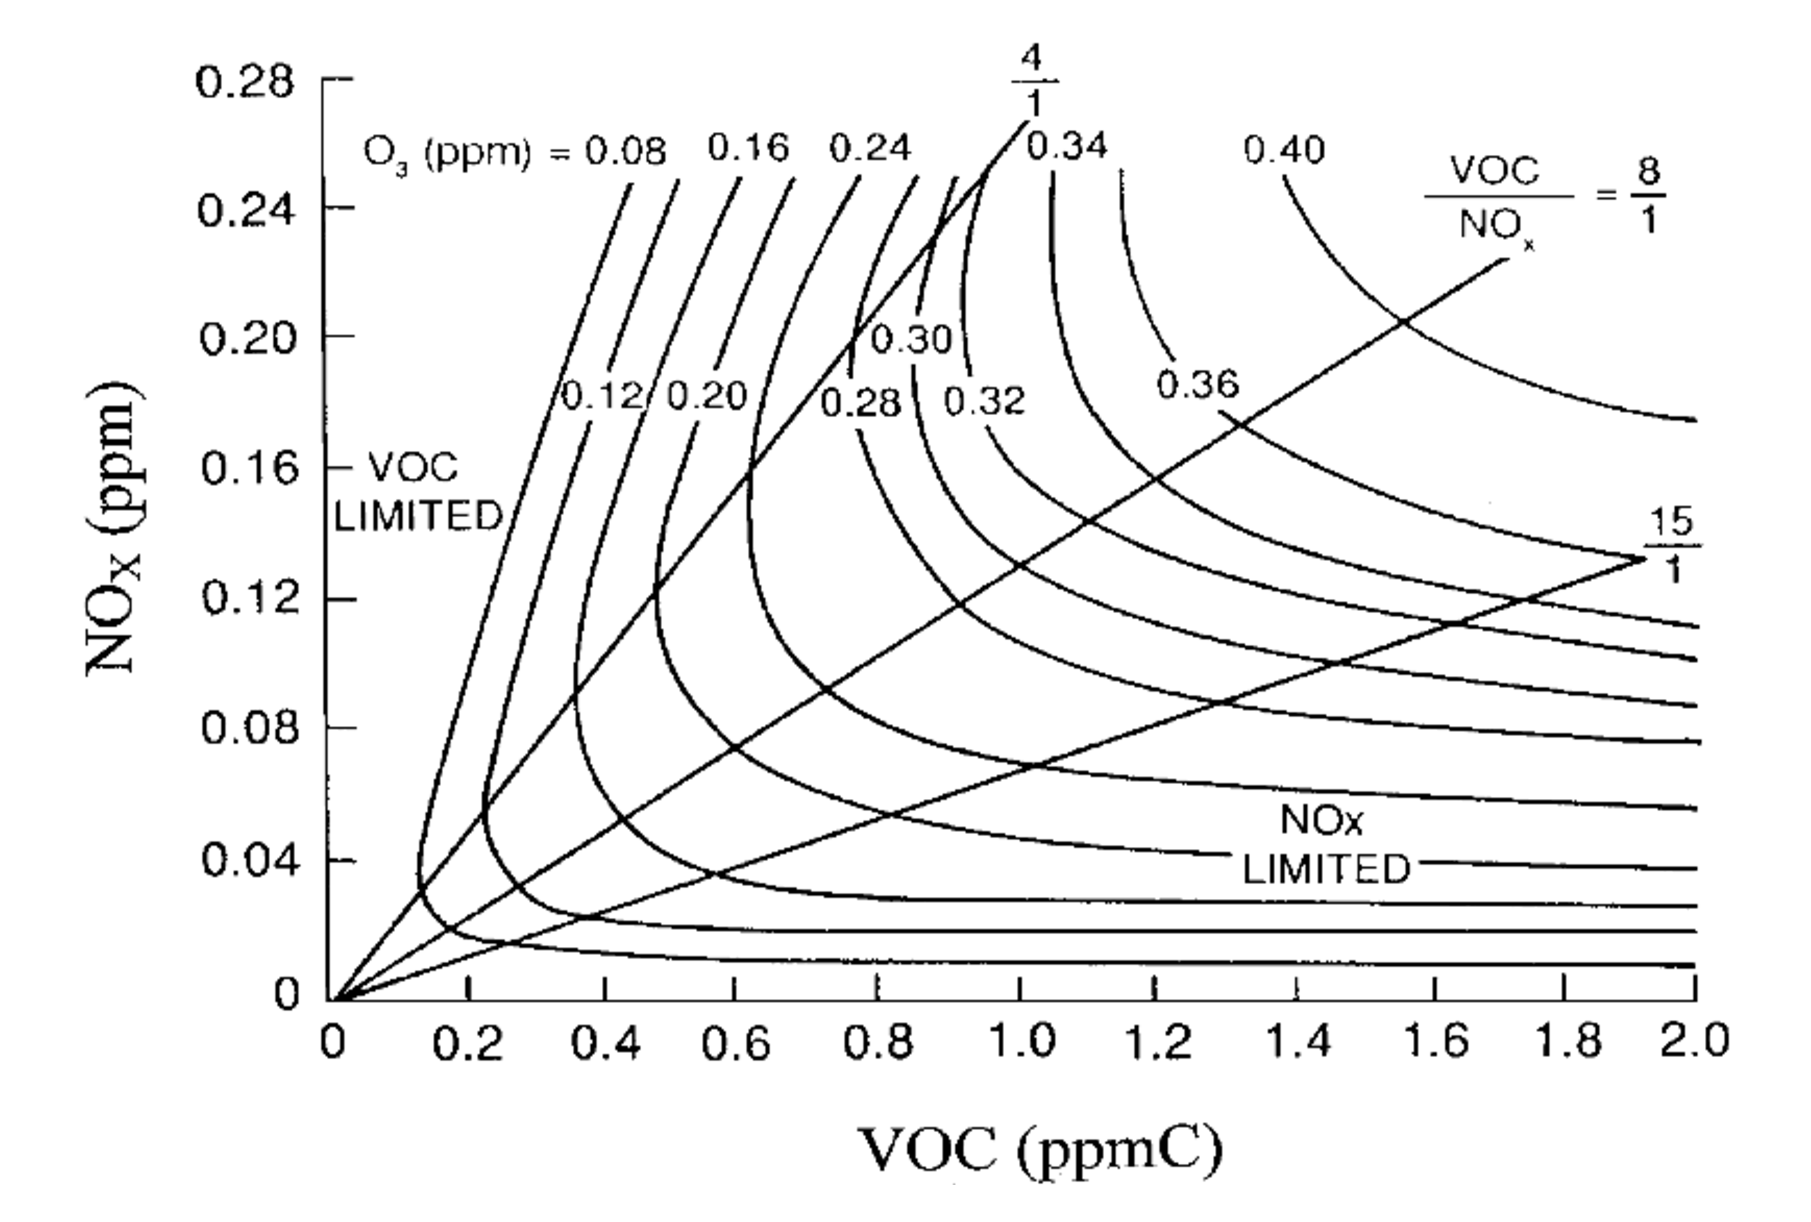
\includegraphics[width = \textwidth]{O3_isopleth}
		\label{f:O3_isopleth}
	\end{center}
\end{figure}
%balance of NOx & NMVOC for O3 production
One of the most important features of ozone production, briefly hinted at prevously, is the dependence of ozone levels on both VOC and \ce{NO_x}.
Figure~\ref{f:O3_isopleth}, from \citet{Jenkin:2000}, depicts the non-linear relationship between \ce{O3} mixing ratios as a function of VOC and \ce{NO_x} mixing ratios.  
This relationship can be divided into distinct regimes of ozone production: \emph{\ce{NO_x}-sensitive} (or \emph{\ce{NO_x}-limited}), \emph{\ce{NO_x}-saturated} (or \emph{VOC-sensitive}) and \emph{VOC-and-\ce{NO_x}-sensitive} regimes. 

The cause of the non-linear relationship is the pathways available to \ce{RO2}.
In the \ce{NO_x}-sensitive regime, the concentration of \ce{NO_x} is low compared to that of radicals hence radicals are more likely to react with other radicals. 
The most common reactions are bimolecular destruction \eqref{r:HO2_OH}, which removes radicals, or combination of radicals \eqref{r:RO2_HO2} into reservoir species that can re-release radicals.
\begin{rxnarray}
    \ce{HO2 + OH} \rightarrow \ce{H2O + O2} \label{r:HO2_OH}
\end{rxnarray}

Reactions between radicals do not directly lead to ozone production as little NO is converted to \ce{NO2}.
Thus increasing \ce{NO_x} would increase the number of NO to \ce{NO2} reactions by peroxy radicals leading to ozone production.
However, increasing VOC levels would not increase \ce{O3} production as increases the likelihood of radical descruction or combination reactions.

The \ce{NO_x}-saturated regime corresponds to high \ce{NO_x} concentrations where radicals will tend to react with \ce{NO_x}. 
Increased \ce{NO_x} levels will not increase \ce{O3} production due to an increase in nitric acid (\ce{HNO3}) formation \eqref{r:NO2_OH}.
Nitric acid is a sink for both OH and \ce{NO_x} removing OH which would otherwise react with emitted VOC to fuel further radical production.
\begin{rxnarray}
    \ce{NO2 + OH} \rightarrow \ce{HNO3} \label{r:NO2_OH}
\end{rxnarray}

The VOC-and-\ce{NO_x}-sensitive regime is characterised by \ce{O3} production being sensitive to both VOC and \ce{NO_x} levels. 
Morever, it is in this atmospheric regime that the maximum amount of ozone is produced and corresponds to the contour ridges in Fig.~\ref{f:O3_isopleth}.
The non-linear relationship can be thought of as a titration process between the amount of radicals and the \ce{NO_x} present in the atmosphere with the VOC-and-\ce{NO_x}-sensitive regime being the turning point \citep{Kleinman:1991, Kleinman:1994}.

This non-linear nature of the troposphere to ozone production makes controlling ozone levels particularly difficult.
The difficulty is exacerbated by the fact that regions can alternate between these regimes depending on the season, time of day etc.
Moreover, fresh emissions tend to occur in the \ce{NO_x}-saturated regime and through transport, the emissions are advected to VOC-and\ce{NO_x}-sensitive and even \ce{NO_x}-sensitive regions.

\subsection{Representing Atmospheric Chemistry in Models} \label{ss:chemistry_models}
Representing this complex chemistry for each emitted VOC in a chemical transport model (CTM) is unrealistic.
Even if all the secondary degradation pathways and products were known for every VOC, a CTM would not be able to efficiently numerically solve the resulting differential equations.
Hence, CTMs use descriptions of atmospheric chemistry that lead to more computationally efficient models.

Not all representations of atmospheric chemistry used in a \emph{chemical mechanism} are prepared in the same way.
For a start, models that also numerically compute meteorology fields require very computationally efficient chemical mechanisms including around $150$ unique species while simpler box models can use chemical mechanisms having many thousands of species.
The simplification techniques used to represent the multitude of VOC and their degradation may lead to discrepancies in the estimations of ozone production.
We compare the ozone production from many reduced chemical mechanisms to a highly detailed chemical mechanism in Sect.~\ref{s:chemical_mechanism_results} and the research questions addressed in this study are framed in Sect.~\ref{s:research_questions}.

\section{Emissions of Ozone Precursors} \label{s:precursor_emissions}
% NOx sources and quantities, weekend effect
\subsection[NOx]{\ce{NO_x}}
Emissions of \ce{NO_x} are mainly through anthropogenic activity.
In the year 2000, almost $52$~Tg~N were emitted with 65~\% through the many forms of fossil fuel combustion \citep{Seinfeld:2006}. 
Examples of fossil fuel combustion that releases \ce{NO_x} are transportation using diesel or petrol vehicles, industrial activities and domestic heating \citep{vonSchneidemesser:2015}.

Up to $95$~\% of \ce{NO_x} emissions from combustion are emitted as NO, which then is oxidised to form \ce{NO2} through \eqref{r:NO_O3} and \eqref{r:RO2_NOb}.
However, due to the increase in diesel vehicles and the implementation of diesel filters the fraction of emitted \ce{NO2} has increased.
\citet{Grice:2009} showed that over Europe, emissions of \ce{NO2} from diesel vehicles has increased from $8.6$~\% in 2000 to $12.4$~\% in 2004.

Despite the overwhelming majority of \ce{NO_x} emissions coming from human activities, there are many important natural sources of \ce{NO_x}.
Lightning and soils are also important sources of \ce{NO_x}, each source contributed about $10$~\% to global \ce{NO_x} emissions in 2000 \citep{Seinfeld:2006}.

\subsection{VOCs}
\subsubsection{Carbon Monoxide}
Carbon monoxide, CO, is emitted directly into the troposphere through combustion and industrial processes.
Another equally-important source of CO, is its chemical formation during the degradation of VOCs.
\citet{Hauglustaine:1998} estimated that globally $881$~Tg~yr$^{-1}$ of CO was produced from chemical oxidation of VOC while $1219$~Tg~yr$^{-1}$ of CO was directly emitted.

Oxidation of CO, through reaction with OH, is its major atmospheric sink and can lead to ozone production.
When the hydroperoxy radical (\ce{HO2}) reacts with NO, \ce{NO2} is formed which may produce ozone and OH is again recycled and available to further oxidise other chemical species.
\begin{rxnarray}
    \ce{CO + OH} & \xrightarrow[]{\ce{O2}} \ce{HO2 + CO2} \label{r:CO_OH} \\
    \ce{HO2 + NO} & \rightarrow \ce{OH + NO2} \label{r:HO2_NO}
\end{rxnarray}

The maximum possible yield of ozone from the degradation of a single molecule of CO occurs when each peroxy radical converts NO to \ce{NO2}.
In this case, a maxmimum of one molecule of ozone can be produced per molecule of CO oxidised.
In reality, this is never achieved as other reactions with the peroxy radicals occur however this is a very informative measure of the \emph{ozone production potential} of a species.

\subsubsection{Methane}
Emissions of methane are between $500$ and $600$~Tg~\ce{CH4}~yr$^{-1}$ with about $60$~\% of the emissions from anthropogenic sources.
The main anthropogenic sources of \ce{CH4} are agriculture, fossil fuels and biomass burning with agriculture contributing $60$~\% of the anthropogenically emitted methane.
Emissions from wetlands are the main natural source of methane emissions \citep{Kirschke:2013}.

Reaction with OH is the main sink of methane and this reaction is important for the concentration of OH in the troposphere.
With increased methane emissions, the concentration of OH will decrease via \eqref{r:CH4_OH} which would lead to a build of methane and other VOCs in the troposphere \citep{Holmes:2013}.
\begin{rxnarray}
    \ce{CH4 + OH} \xrightarrow[]{\ce{O2}} \ce{CH3O2 + H2O} \label{r:CH4_OH}
\end{rxnarray}

The secondary degradation of methane produces the methylperoxy radical \ce{CH3O2} as well as \ce{HO2} as well as CO.
Assuming that every peroxy radical converts NO to \ce{NO2} then methane degradation can produce a maximum five molecules of \ce{O3} per molecule of \ce{CH4} oxidised.
Methane (\ce{CH4}) has a lifetime of about $9$~years, significantly longer than all other VOCs.
Thus, methane influences ozone production on the global rather than the regional scale.  

\subsubsection{Non-Methane VOCs}
%VOCs, types of VOCs and source (A vs B)
A wide variety of non-methane VOC (NMVOC) are emitted from anthropogenic activities directly into the troposphere.
Solvent use, industry, fossil fuel burning and transportion are all major activities emitted NMVOCs of varying functional groups and carbon numbers.
The maximum number of molecules of \ce{O3} produced per degradation of an emitted NMVOC depends on the number of NO to \ce{NO2} conversions by the peroxy radicals formed during the degradation of the NMVOC.
This is highly dependent on the type of NMVOC and the number of carbons in the NMVOC.

Many NMVOCs emitted from anthropogenic sources are also hazardous to human health in their own right.
For example, benzene and formaldehyde are suspected carcinogens \citep{Laurent:2014}.
It is also worthwhile to note that the NMVOC thought to be the most hazardous to human health do not correspond to NMVOC that have a high ozone production potential.

Globally, \citet{Lamarque:2010} estimated that $130$~Tg~NMVOC were emitted from anthropogenic sources in the year 2000.
This amount is dwarfed by the total emissions from biogenic sources -- $1000$~Tg~NMVOC~yr$^{-1}$, almost eight times the amount of NMVOC emitted from anthropogenic sources \citep{Guenther:2012}.

Of the NMVOC emitted from vegetation, isoprene (\ce{C5H8}) dominates at the global scale however emissions of monoterpenes and sesquiterpenes are also significant.
There is typically overlap in the NMVOC species emitted from biogenic and anthropogenic sources. 
For example, isoprene has also been measured in the urban areas of London and Paris away from direct emission sources and since isoprene is a very reactive NMVOC it is unlikely to be transported from outside the area, there appears to be anthropogenic sources of isoprene \citep{vonSchneidemesser:2011}.
Also many small NMVOC that are typically emitted from anthropogenic sources, such as methanol and acetaldehyde, are also emitted from vegetation \citep{Guenther:2012}.

The NMVOC species emitted vary between types of vegetation -- some trees emit large amounts of isoprene while others do not.
Also, the quantity of NMVOC emissions from vegetation depends on atmospheric (such as, temperature and radiation) and biological variables (such as, leaf age and leaf area index).
Thus only regulation of NMVOC from anthropogenic sources is possible and drastic reductions in anthropogenic \ce{NO_x} are required to minimise the burden of the population to ozone pollution.
Areas dominated by biogenic NMVOC emissions and away from large \ce{NO_x} sources (\ce{NO_x}-sensitive regime) could lead net loss of ozone through direct reactions of ozone with many biogenic NMVOC and the net loss of radicals (discussed in Sect.~\ref{ss:VOC&NOx}).

\subsection{Representing VOC Emissions in Models}
%representation of VOC emissions in models using emission inventories
Representing the multitude of emitted VOCs, from either anthropogenic or biogenic sources is one of the major challenges of the modelling community.
Models use emission inventories that specify the type and quantity of VOCs emitted over a region or even the whole globe.
However, as hinted at, this is no easy task and emission inventories are one of the major sources of uncertainty of the model input \citep{Russell:2000}.

Emission inventories typically specify emissions for \ce{NO_x}, CO, \ce{CH4}, NMVOC as well as non-gas-phase emissions such as particulate matter.
Emissions are assigned to source sectors, called SNAP (Standardised Nomenclature for Air Pollutants) sectors, such as those listed in Table~\ref{t:SNAP}.
The rest of this section shall discuss specifications of NMVOC emissions from emission inventories.

\begin{table}
    \centering
    \caption[SNAP sectors in the TNO\_MACCIII]{SNAP sectors for anthropogenic emissions listed in the TNO\_MACCIII inventory \citep{Kuenen:2014}.}
    \begin{tabular}{cl}
        \hline \hline
        \textbf{SNAP Sector} & \textbf{Description} \\
        \hline \hline
        1 & Public Power \\
        2 & Residential Combustion \\
        34 & Industry \\
        5 & Fossil Fuel \\
        6 & Solvent Use \\
        71 & Road Transport: Gasoline \\
        72 & Road Transport: Diesel \\
        73 & Road Transport: Others \\
        74 & Road Transport: Evaporation \\
        75 & Road Transport: Wear \\
        8 & Non-road Transport \\
        9 & Waste \\
        10 & Agriculture \\
        \hline \hline
    \end{tabular}
    \label{t:SNAP}
\end{table}

%temporal profile of emissions
Emissions of both \ce{NO_x} and VOCs are not constant over the year, month or time of day.
In many regions, a noticible reduction in \ce{NO_x} emissions, due to reduced road transport, is noted during the weekend -- called the ``weekend-effect''.
The weekend-effect has implications on the ozone production during the weekend.
For example, ozone production is \ce{NO_x}-saturated during weekdays in San Joaquin Valley, California.
The reduction of \ce{NO_x} emissions during the weekend moves ozone production to the VOC-and-\ce{NO_x} sensitive regime, hence higher ozone levels are measured during the weekend \citep{Pusede:2014}.

Anthropogenic NMVOC emissions from the different SNAP sectors also have a temporal distribution.
Many SNAP sectors, such as industry and solvent use, have a reduction in emissions on weekends.
Transport emissions tend to peak during the morning and evening rush hours and emissions due to solvent have a strong diurnal cycle.
Residential combustion tends to be highest during the winter months and lowest during the summer \citep{Gon:2011}.

Emission factors are assigned to the emissions from SNAP categories to represent the temporal profiles within a model.
Biogenic VOC emissions are typically estimated using an algorithm including variables on which BVOC emissions are dependent.
MEGAN2.1 \citep{Guenther:2012} is commonly used by the modelling community to represent emissions from nature.
The MEGAN2.1 model utilised variables such as temperature and radiation levels which are calculated during model simulations and then fed into the MEGAN2.1 model to estimate BVOC emissions.

%emissions in models - lumping
One issue for the modelling community with using emission inventories for specifying NMVOC emissions is translating the listed emissions into the chemical species used by the chemical mechanism.
Emission inventories are not normally immediately available for use with a chemical mechanism which can lead to different modelling groups allocating the emission inventory input differently for the same chemical mechanism \citep{Carter:2015}.
Chemical mechanisms used in global and regional models cannot represent each NMVOC individually for reasons of computational efficiency thus many NMVOCs must be represented by the particular lumped (or aggregated) species of the chemical mechanism.
This translation into lumped species differs between chemical mechanisms (Sect.~\ref{ss:chemistry_models}).
The effect that lumping emissions of NMVOC into different chemical mechanism has on simulated ozone production is explored in this work in Sect.~\ref{s:EI_results}.

\section{Effects of Meteorology on Ozone Production} \label{s:meteo_ozone}

The effect of meteorology is an aspect of atmospheric chemical transport modelling that needs to be taken into account. 
However it is also frequently the major source of uncertainty for the calculated \ce{O3} concentrations. 
Wind speeds in particular may lead to under- or over-predicated values of \ce{O3} concentrations \citep{Sillman:1999}. 

Discuss effects of meteorology on reservoir species which influences ozone production.

\section{Research Questions} \label{s:research_questions}

